\documentclass[12pt]{article} 
\usepackage[utf8]{inputenc}
\usepackage{geometry}
\geometry{letterpaper}
\usepackage{graphicx} 
\usepackage{parskip}
\usepackage{booktabs}
\usepackage{array} 
\usepackage{paralist} 
\usepackage{verbatim}
\usepackage{subfig}
\usepackage{fancyhdr}
\usepackage{sectsty}

\pagestyle{fancy}
\renewcommand{\headrulewidth}{0pt} 
\lhead{}\chead{}\rhead{}
\lfoot{}\cfoot{\thepage}\rfoot{}

%%% SECTION TITLE APPEARANCE
\allsectionsfont{\sffamily\mdseries\upshape} 

%%% ToC (table of contents) APPEARANCE
\usepackage[nottoc,notlof,notlot]{tocbibind} 
\usepackage[titles,subfigure]{tocloft}
\renewcommand{\cftsecfont}{\rmfamily\mdseries\upshape}
\renewcommand{\cftsecpagefont}{\rmfamily\mdseries\upshape} %

\usepackage{amsmath}
\usepackage{amssymb}

\title{APMA 0350: Applied Ordinary Differential Equations}
\author{Milan Capoor}
\date{Fall 2022}

\begin{document}
\maketitle
\section{Lecture 1: What is a differential equation?}
\subsection*{Part I - Introduction to the course}
\begin{itemize}
    \item Professor Peyam Tabrizian 
    \item Office Hours Tu 12:15-1:15 pm, Th and F 1:15-2:15
    \item Youtube: https://www.youtube.com/c/DrPeyam/community
\end{itemize}

\subsection*{Part II - What is a Differential equation?}
A differential equation (ODE) is an equation that involves one or more
derivatives of a function y

Examples:
\begin{enumerate}
    \item $y' =2y$ 
    \item $y'' + 5y' + 6y = 0$
    \item $(y''')^2 = \sin (y^3) + y+ t^2$ (where t is independent variable)
    \item $\begin{cases}
        x'(t) = 2x(t) - 3y(t)\\
        y'(t) = 5x(t) + 6y(t)
    \end{cases}$
    \item Partial differential equations (studies in APMA 0360): $\frac{d^2 u}{dx\, dt} + u = \left(\frac{du}{dx}\right)^2$
\end{enumerate}

Applications:
ODEs are used to model and describe many types of processes
\begin{enumerate}
    \item Biology (epidemiology, ecology, cancer research, COVID)
    \item Climate Research (flooding and wildfires)
    \item Economics (stock market, options pricing, wealth and income
    distribution)
    \item Engineering and Physics (from mass-spring systems to aircraft
    design)
    \item Neuroscience and Computer Science (models of brain activity
    patterns, deep learning networks, traffic control)
    \item Modeling outbreak of a Zombie Attack
    \item Chemical Reactions (the PDE that got the PhD!)
\end{enumerate}

From Peyam's PhD advisor:
“If you can solve all differential equations, then you can solve the universe.” $\implies$ DiffEqs are hard to solve but each equation is like its own universe 

\subsection*{Part III - The most basic example}
Example 1: Solve $y' = 2y$ with $y(0) = 3$

Solution:
\begin{enumerate}
    \item Isolate y
    \[y' = 2y \implies \frac{y'}{y} = 2\]

    \item Recognise that the LHS is a derivatives
    \[(\ln |y|)' = 2\]
    \[\ln |y| = 2t + C\]
    \[|y| = e^{2t + C} = e^Ce^{2t}\]
    \[y = \pm e^C e^{2t} = Ce^{2t}\]

    \item Initial condition
    \[y(0) = 3 \implies Ce^0 = 3 \implies C = 3\]
    \[\boxed{y(t) = 3e^{2t}}\]
\end{enumerate}

\textbf{Fact:}
The general solution of $y' = ky$ is 
\[\boxed{y(t) = Ce^{kt}}\]

\subsection*{Part IV - Classification}
\emph{Order:} the highest derivative that appears

Example: 
\begin{enumerate}
    \item $y' = 2y + 1$ is first-Order
    \item $y'' + 5y'+ 6y = 0$ is second-order (second derivative)
    \item $t^5 y''' - 4y' + y = t^3$ is third-order
\end{enumerate}

\emph{Homogeneous:} if the right hand side is 0
\emph{Inhomogeneous:} the right hand is not 0
\begin{enumerate}
    \item $y'' + 5y; + 6y = 0$ is homogeneous
    \item $y'' + 5y' + 6y = t^2$ is inhomogeneous
    \item $y'' + 5y' + 6y + 2t = 2t$ is homogeneous (the 2t terms cancel)
\end{enumerate}

Classifications of ODEs (from easiest to hardest):
\emph{Constant coefficient:}
\begin{enumerate}
    \item $y'' + 5y' + 6y = 0$
    \item $y'' + 5t' + 6y = e^{2t}$
    \item NOT $t^2 y'' + 2y' + 3y = 0$
\end{enumerate}

\emph{Linear DE:} the coefficients can depend on t but not on y
\begin{enumerate}
    \item $y' + ty = 0$
    \item $t^2 y'' + \sin t y' + 2y = 0$
    \item $y'' + 5y' + 6y = 3$
\end{enumerate}

\section{A summary of the first half of the course, the notes for which were lost:}
\subsection*{Lecture Sep 9: Direction Fields}

\emph{Direction field:} A way of qualitatively studying the behaviour of an ODE by plotting the tangent lines at each point. When you draw a line through a point, following the slope arrows, you create a plot of the ODE's solution with that point as the initial condition
- Can be generated with the dfield app (https://aeb019.hosted.uark.edu/dfield.html)

\subsection*{Lecture Sep 12: Qualitative methods}

\emph{Autonomous ODE:} the right-hand-side doesn't depend on t
Special case: Logistic equation $y = \alpha y (1 - \frac{y}{\beta})$
Where $\alpha$ is the growth rate and $\beta$ is the limiting factor. 

\emph{Equilibrium Solutions:} the lines where $f(y) = 0$
To determine what happens at these solutions, we draw a \emph{bifurcation diagram}

For the logistic equation $y= 3y (1 - \frac{y}{20})$, the bifurcation diagram is 
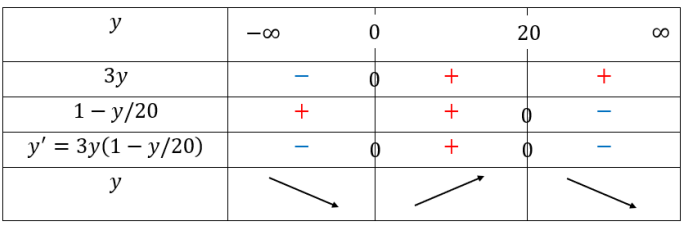
\includegraphics{Images/bifurcation.png}

Which gives us the graph 
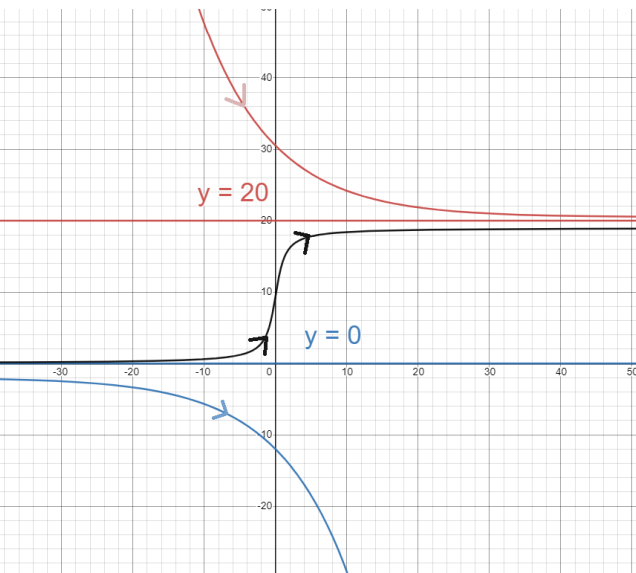
\includegraphics{Images/logistic graph.png}

Classifying solutions:
\begin{itemize}
    \item If the solutions go towards an equiblibrium point from each side, it is \emph{stable}
    \item If the solutions move away, it is \emph{unstable}
    \item If the solutions approach from one side and are repelled from the other, it is \emph{bistable}
\end{itemize}

\subsection*{Lecture Sep 14: Existence and uniqueness}
\emph{Existence and Uniqueness Theorem:}
Given $(t_0, y_0)$, consider the ODE 
\[\begin{cases}
    y' = f(y, t)\\
    y(t_0) = y_0
\end{cases}\]
If $f$ and $f_y = \partial f / \partial y$ are continuous near $(t_0, y_0)$, then the ODE has a unique solution $y = y(t)$ for some $t \in (-\delta, \delta), \; \delta > t_0$
\section{Lecture: Oct 21}
\subsection*{Part I - Classifying Equilibrium Points of Nonlinear ODEs}
Example 1: Classify the equilibrium points of 
\[\begin{cases}
    x' = -x + xy\\
    y' = -8y + 4xy
\end{cases}\]

To find the equilibrium points, set $x' = 0$ and $y' = 0$

In this equation,
\[\begin{cases}
    x' = -x(1 - y) = 0\\
    y' = -y(8 - 4x) = 0
\end{cases} \implies (0, 0) \quad (2, 1)\]

Linearization:
\[\nabla F(x, y) = \begin{bmatrix}
    \frac{\partial (-x + xy)}{\partial x} & \frac{\partial (-x + xy)}{\partial y}\\
    \frac{\partial (-8y + 4xy)}{\partial x} & \frac{\partial (-8y + 4xy)}{\partial y}\\
\end{bmatrix} = \begin{bmatrix}
    -1 + y & x\\
    4y & -8 + 4x
\end{bmatrix}\]

Case 1: $(0, 0)$
\[\nabla F(0, 0) = \begin{bmatrix}
    -1 & 0\\
    0 & -8
\end{bmatrix}\]

The eigenvalues of this are $\lambda = -1$ and $\lambda = - 8$, both of which are less than zero so the solution is a sink and the point $(0, 0)$ is \textbf{stable}.

Note: For a complex negative eigenvalue (e.g. $\lambda = -2 + 3i$), there will be a spiral sink which is also stable

Case 2: $(2, 1)$
\[\nabla F(2, 1) = \begin{bmatrix}
    0 & 2\\
    4 & 0
\end{bmatrix}\]

Eigenvalues:
\[\lambda^2 - 8 = 0 \implies \lambda = \pm 2\sqrt{2}\]

In this case, one eigenvalue is positive and the other is negative so this is a \textbf{semi-stable saddle point}

Stability cases summary:
\begin{itemize}
    \item If the eigenvalues are both negative, we have a sink
    \item If both positive, unstable
    \item If one positive and one negative, saddle point
    \item If 0, "screwed"
\end{itemize}

\subsection*{Part II - Application Number 1: Competing Species}
Recall: Logistic equation 
\[y' = 3t \left(1 - \frac{y}{20}\right)\]
(the growth of a population with limited resources, where 3 is the growth rate and 20 is the limiting factor)

Guiding question: What if you have two coexisting animal species?
\[\begin{cases}
    x(t) = \text{ population of rabbits}\\
    y(t) = \text{ population of sheep}\\
\end{cases}\]

Note: The two species do not prey on each other but compete for the same limited resources 

\begin{enumerate}
    \item Logistic Approach:
    \[\begin{cases}
        x' = 3x(1 - \frac{x}{1.5})\\
        y' = 2y(1 - \frac{y}{2})
    \end{cases} = \begin{cases}
        x' = 3x - 2x^2\\
        y' = 2y - y^2
    \end{cases}\]
    
    However, this model does not account for competition for limited resources
    
    \item A better model!
    \[\begin{cases}
        x' = 3x - 2x^2 - xy\\
        y' = 2y - y^2 - xy
    \end{cases}\]
    Here, the xy term accounts for the interaction between the two populations 
    (if either were 0, the term would go to zero)
\end{enumerate}

\subsection*{Part III - Equilibria}
Example 2: Find the equilibrium points of the model 
\[\begin{cases}
    x' = x(3 - 2x - y) = 0\\
    y' = y(2 - y - x) = 0
\end{cases}\]

\[\begin{cases}
    x = 0 \implies y = \{0, 2\} \implies \boxed{(0, 0) \quad (0, 2)}\\
    3 - 2x - y = 0 \implies (y = 0 \implies x = \frac{3}{2}) \\
    \text{ OR } \left(2-y-x = 0 \implies \begin{cases}
        3 - 2x - y = 0\\
        2 - y- x = 0
    \end{cases} \implies x = 1, \quad y = 1\right) \implies \boxed{(\frac{3}{2}, 0) \quad (1, 1)}
\end{cases}\]

Thus, the four possible outcomes:
\begin{enumerate}
    \item $(0, 0)$ - Both die 
    \item $(0, 2)$ - Sheep win
    \item $(\frac{3}{2}, 0)$ - Bunnies win 
    \item $(1, 1)$ - Coexistence
\end{enumerate}

To classify each point, we use the linearization:
\[\nabla F(x, y) = \begin{bmatrix}
    \frac{\partial (3x - 2x^2 0 xy)}{\partial x} & \frac{\partial (3x - 2x^2 0 xy)}{\partial y}\\
    \frac{\partial (2y - y^2 - xy)}{\partial x} & \frac{\partial (2y- y^2 - xy)}{\partial y}
\end{bmatrix} = \begin{bmatrix}
    3 - 4x - y & -x\\
    -y & 2 - 2y - x
\end{bmatrix}\]

Thus,
\begin{enumerate}
    \item $F(0, 0) = \begin{bmatrix}
        3 & 0 \\
        0 & 2
    \end{bmatrix} \implies \lambda = \{3, 2\} \implies$ the system is unstable 
    \item $F(0, 2) = \begin{bmatrix}
        1 & 0\\
        -2 & -2
    \end{bmatrix} = \lambda = \{1, -2\} \implies$ the system is semistable so the sheep will survive
    \item $F(\frac{3}{2}, 0) = \begin{bmatrix}
        -3 & -\frac{3}{2}\\
        0 & \frac{1}{2}
    \end{bmatrix} \implies \lambda = \{-3, \frac{1}{2}\} \implies $ the system is also a saddle so the bunnies survive
\end{enumerate}

\section{Lecture: Oct 24}
\subsection*{Part I - Rabbits and Sheep Model Recap}
Our model, where x is the population of rabbits and y is the population of sheep:
\[\begin{cases}
    x' = 3x - 2x^2 - xy\\
    y' = 2y - y^2 - xy
\end{cases}\]

Equilibrium points: $(0, 0), \; (0, 2), \; (\frac{3}{2}, 0),\; (1, 1)$

\subsection*{Part II - Classification continued}
\[\nabla F(x, y) = \begin{bmatrix}
    3 - 4x - y & -x\\
    -y & 2 - 2y - x
\end{bmatrix}\]
"Again, this is applied math. There is no reason we add this term. It just works. And if it doesn't, we work harder and make up a different term that just works"

\[\nabla F(1, 1) = \begin{bmatrix}
    -2 & -1\\
    -1 & -1
\end{bmatrix}\] 

Eigenvalues:
\[| A - \lambda I | = (-2 - \lambda)(-1 - \lambda) - 1 = \lambda^2 + 3 \lambda + 1 = 0\]
\[\lambda = \frac{-3 \pm \sqrt{9 - 4(1)}}{2} = -\frac{3}{2} \pm \frac{\sqrt{5}}{2}\]

Here, both eigenvalues are negative so (1, 1) is stable

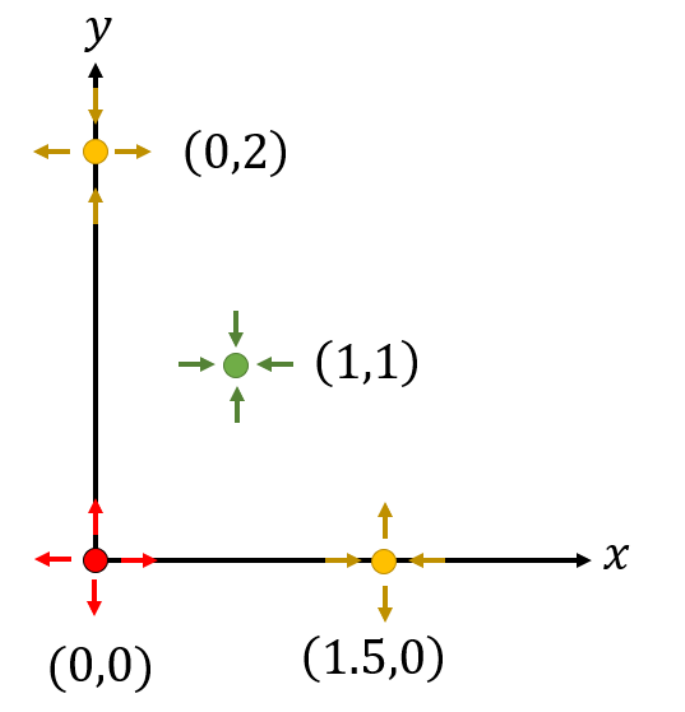
\includegraphics{Images/rabbits and bunnies plot.png}

Note: We do not know which directions of the saddle are positive and which are negative

To draw the rest of the picture, we need to the region $x \in [0, \frac{3}{2}]$ and $y \in [0, 2]$ because those coordinates are the limiting factors of the system 

\subsection*{Part III - Nullclines}
We want to study the behavior of solutions on the axes $x = 0, y = 0, x = 1.5, y = 2$

\emph{Nullclines:} axes where x' or y' is 0

\begin{itemize}
    \item Case 1: $x = 0$ (no rabbits)
        \[\begin{cases}
            x' = 0\\
            y' = 2y - y^2
        \end{cases}\]
        As a result, we are only concerned with vertical movement on the axis.

        Looking at the sign of y', we see that it will be positive $[0, 2]$ and negative $[2, \infty]$

        Therefore, the arrows will be moving up on the y-axis up to 2 and decreasing above 2, so we also now know the orientation of the saddle point.

        Interpretation: if there are no rabbits, the population of sheep will simply increase until they hit their own carrying capacity (which is exactly what we expect!)

    \item Case 2: $y = 0$ (no sheep)
    \[\begin{cases}
        x' = 3x - 2x^2\\
        y' = 0
    \end{cases}\]
    So x will increase until it reaches $x = \frac{3}{2}$

    \item Case 3: $y = 2$ (sheep reached limiting pop)
        \[\begin{cases}
            x' = x - 2x^2\\
            y' = -2x
        \end{cases}\]

        The sign of y' is negative, so on this axis the arrows are pointing down. And, because x' is positive $[0, \frac{1}{2}]$ and negative $[\frac{1}{2}, 1.5]$, the arrows also point roughly towards the centre of the region 

    \item Case 4: $x = 1.5$ (saddle)
        \[\begin{cases}
            x' = - \frac{3}{2}y\\
            y' = \frac{1}{2}y - y^2
        \end{cases}\]

        The sign of x' is negative so the arrows point to the left, and y' is positive on $[0, \frac{1}{2}]$ and negative $[\frac{1}{2}, 2]$
\end{itemize}

From all of this, we can fill in the graph from earlier and draw a few solutions:

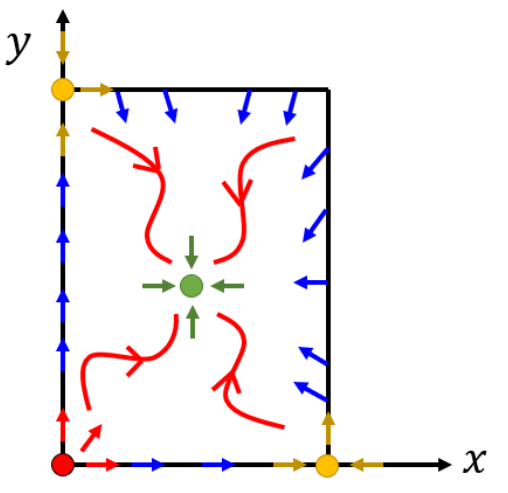
\includegraphics{Images/rabbits and bunnies plot 2.png}

Epic conclusion: the species will not go extinct! they will happily coexist and eventually reach the equilibrium (1, 1)

BUT: we missed the case where there is a periodic orbit around the equiblibrium point and where the two species struggle for eternity

\subsection*{Part IV - Periodic Orbits}
To rule out the possibility of periodic orbits, we just need to examine the behaviour of the sysytem at the axes of the equilibrium point.

\begin{itemize}
    \item Case 1: $x = 1$
    \[\begin{cases}
        x' = 2x - 2x^2\\
        y' = 1 - x
    \end{cases}\]

    So on the axis $y = 1$, if $x < 1$, the arrows are pointing up, and if $x > 1$, they are pointing down.

    \item Case 2: $y = 1$
    \[\begin{cases}
        x' = 1 -y\\
        y' = -y + y^2
    \end{cases}\]
    So on the axis x = 1, if y < 1, the arrows are pointing to the right (increasing) and if y > 1, they are pointing to the left (x decreasing)
\end{itemize}

Completing the picture, we see that no periodic orbit is possible!

\section{Lecture: Oct 26}
\subsection*{Part I - Chemical Tanks}
Assume there are three chemical tanks in series.
\begin{itemize}
    \item Tank 1: $Q_1(t)$ kg salt, 2L water
    \item Tank 2: $Q_2(t)$ kg salt, 4L water
    \item Tank 3: $Q_3(t)$ kg, 3L water
    \item The first tank has an input of 6L/min of water and 1/3 kg/L salt 
    \item Each minute, 4L salinated water flows from the first tank to the second and from the second to the third
    \item The third tank has an output of 12 L/min
\end{itemize}

Set up a system in the form $Q'(t) = AQ(t) + b$

\begin{enumerate}
    \item $Q'_1(t) = 6 (\frac{1}{3}) - 4 \left(\frac{Q_1(t)}{2}\right) = 2 - 2 Q_1(t)$
    \item $Q_2'(t) = 4 \left(\frac{Q_1(t)}{2}\right) - 4\left(\frac{Q_2(t)}{4}\right) = 2Q_1(t) - Q_2(t)$
    \item $Q_3'(t) = 4\left(\frac{Q_2(t)}{4}\right) - 12\left(\frac{Q_2(t)}{3}\right) = Q_2(t) - 4Q_3(t)$
\end{enumerate}

So, the system is 
\[\begin{cases}
    Q_1' = -2Q_1 + 2\\
    Q_2' = 2Q_1 - Q_2
    Q_3' = Q_2 - 4Q_3
\end{cases}\]

So,
\[Q' = \begin{bmatrix}
    -2 & 0 & 0\\
    2 & -1 & 0\\
    0 & 1 & -4
\end{bmatrix} Q(t) + \begin{bmatrix}
    2\\0\\0
\end{bmatrix}\]

\subsection*{Part II - Matrix Exponentials}
Example 2: Use matrix exponentials to solve $x' = Ax$ where 
\[A = \begin{bmatrix}
    7 & -1\\
    9 & 1
\end{bmatrix}, \quad x(0) = \begin{bmatrix}
    2\\3
\end{bmatrix}\]

Solution:
\[\begin{vmatrix}
    7 - \lambda & -1\\
    9 & 1 - \lambda
\end{vmatrix} = (7 - \lambda)(1 - \lambda) + 9 = \lambda^2 - 8\lambda + 16 = 0\]
\[(\lambda - 4)^2 = 0 \implies \lambda = 4\]

\[e^{At} = e^{4t} e^{(A - 4I)t} = e^{4t} (I + (A - 4I)t)\]
\[e^{4t} \left(\begin{bmatrix}
    1 & 0\\
    0 & 1
\end{bmatrix} + t\begin{bmatrix}
    3 & -1\\
    9 & -3
\end{bmatrix}\right)\]
\[= e^{4t} \begin{bmatrix}
    1 + 3t & -t\\
    9t & 1 - 3t
\end{bmatrix}\]

\[x(t) = C_1 e^{4t} \begin{bmatrix}
    1 + 3t\\
    9t
\end{bmatrix} + C_2 e^{4t} \begin{bmatrix}
    -t\\
    1 - 3t
\end{bmatrix}\] 

\[x(0) = \begin{bmatrix}
    2\\3
\end{bmatrix} = C_1\begin{bmatrix}
    1\\
    0
\end{bmatrix} + C_2 \begin{bmatrix}
    0\\1
\end{bmatrix} \implies C_1 = 2, \quad C_3 = 3\]

\[x(t) = 2e^{4t}  \begin{bmatrix}
    1 + 3t\\
    9t
\end{bmatrix} + 3e^{4t} \begin{bmatrix}
    -t\\
    1 - 3t
\end{bmatrix} = \boxed{e^{4t} \begin{bmatrix}
    2 + 3t\\
    3 + 9t
\end{bmatrix}}\]

\subsection*{Part III - Euler's Method}
Example 3: Apply Euler's method with N = 2 to find $y_0, y_1, y_2$ on $[2, 6)$ where
\[\begin{cases}
    y' = y^2 - 2t\\
    y(2) = 1
\end{cases}\]

Solution:
\[h = \frac{6 - 2}{2} = 2\]
\begin{align*}
    y_0 = 1\\
    y_1 = y_0 + h y'(2) = 1 + 2 (1 - 4) = -5\\
    y_2 = y_1 + h y'(4) = -5 + 2 (25 - 8) = -5 + 34 = 29
\end{align*}

\subsection*{Part IV - Phase Portraits}
Example 4: Sketch the phase portrait of $x' = Ax$ where
\[A = \begin{bmatrix}
    3 & 4\\
    -1 & 3
\end{bmatrix}\]

Solution:
\[\lambda = 3 \pm 2i\]
\[\vec{v}_{3 + 2i} = \begin{bmatrix}
    -2i\\
    1
\end{bmatrix}\] 

\[e^{(3 + 2i)t} \begin{bmatrix}
    -2i\\
    1
\end{bmatrix} = e^{3t} \left(\cos (2t) + i \sin (2t)\right) \left(\begin{bmatrix}
    0\\
    1
\end{bmatrix} - i \begin{bmatrix}
    2\\0
\end{bmatrix}\right)\]

\[x(t) = C_1 \left(e^{3t} \cos (2t) \begin{bmatrix}
    0\\1
\end{bmatrix} + \sin(t) \begin{bmatrix}
    2\\0
\end{bmatrix}\right) + C_2 e^{3t} \left(\cos(2t) \begin{bmatrix}
    -2\\
    0
\end{bmatrix} + \sin (2t) \begin{bmatrix}
    0\\1
\end{bmatrix}\right)\]
\end{document} 